% This file was converted to LaTeX by Writer2LaTeX ver. 1.0.2
% see http://writer2latex.sourceforge.net for more info
\documentclass[twoside,letterpaper]{article}
\usepackage[latin1]{inputenc}
\usepackage[T1]{fontenc}
\usepackage[english]{babel}
\usepackage{amsmath}
\usepackage{amssymb,amsfonts,textcomp}
\usepackage{color}
\usepackage{array}
\usepackage{supertabular}
\usepackage{hhline}
\usepackage{hyperref}
\usepackage{multirow}
\hypersetup{pdftex, colorlinks=true, linkcolor=blue, citecolor=blue, filecolor=blue, urlcolor=blue, pdftitle=SYSTEMS AND SOFTWARE REQUIREMENTS SPECIFICATION (SSRS) TEMPLATE, pdfauthor=Clinton Jeffery, pdfsubject=, pdfkeywords=}
\usepackage[pdftex]{graphicx}
% Outline numbering
\setcounter{secnumdepth}{5}
\renewcommand\thesection{\arabic{section}}
\renewcommand\thesubsection{\arabic{section}.\arabic{subsection}}
\renewcommand\thesubsubsection{\arabic{section}.\arabic{subsection}.\arabic{subsubsection}}
\renewcommand\theparagraph{\arabic{section}.\arabic{subsection}.\arabic{subsubsection}.\arabic{paragraph}}
\renewcommand\thesubparagraph{\arabic{section}.\arabic{subsection}.\arabic{subsubsection}.\arabic{paragraph}.\arabic{subparagraph}}
\makeatletter
\newcommand\arraybslash{\let\\\@arraycr}
\makeatother
% Page layout (geometry)
\setlength\voffset{-1in}
\setlength\hoffset{-1in}
\setlength\topmargin{0.5in}
\setlength\oddsidemargin{1in}
\setlength\evensidemargin{1in}
\setlength\textheight{8.278in}
\setlength\textwidth{6.5in}
\setlength\footskip{0.561in}
\setlength\headheight{0.5in}
\setlength\headsep{0.461in}
% Footnote rule
\setlength{\skip\footins}{0.0469in}
\renewcommand\footnoterule{\vspace*{-0.0071in}\setlength\leftskip{0pt}\setlength\rightskip{0pt plus 1fil}\noindent\textcolor{black}{\rule{0.25\columnwidth}{0.0071in}}\vspace*{0.0398in}}
% Pages styles
\makeatletter
\newcommand\ps@Standard{
  \renewcommand\@oddhead{\selectlanguage{english}\rmfamily\color{black} University of Idaho CS Department Instructional Use\hfill \hfill NOT FOR RELEASE}
  \renewcommand\@evenhead{\@oddhead}
  \renewcommand\@oddfoot{\foreignlanguage{english}{\textcolor{black}{SSRS Page }}\foreignlanguage{english}{\textcolor{black}{\thepage{}}}}
  \renewcommand\@evenfoot{\@oddfoot}
  \renewcommand\thepage{\arabic{page}}
}
\newcommand\ps@Convertviii{
  \renewcommand\@oddhead{}
  \renewcommand\@evenhead{\@oddhead}
  \renewcommand\@oddfoot{}
  \renewcommand\@evenfoot{\@oddfoot}
  \renewcommand\thepage{\arabic{page}}
}
\newcommand\ps@Convertvii{
  \renewcommand\@oddhead{}
  \renewcommand\@evenhead{\@oddhead}
  \renewcommand\@oddfoot{}
  \renewcommand\@evenfoot{\@oddfoot}
  \renewcommand\thepage{\arabic{page}}
}
\newcommand\ps@Convertvi{
  \renewcommand\@oddhead{}
  \renewcommand\@evenhead{\@oddhead}
  \renewcommand\@oddfoot{}
  \renewcommand\@evenfoot{\@oddfoot}
  \renewcommand\thepage{\arabic{page}}
}
\newcommand\ps@Convertv{
  \renewcommand\@oddhead{}
  \renewcommand\@evenhead{\@oddhead}
  \renewcommand\@oddfoot{}
  \renewcommand\@evenfoot{\@oddfoot}
  \renewcommand\thepage{\arabic{page}}
}
\newcommand\ps@Convertiv{
  \renewcommand\@oddhead{}
  \renewcommand\@evenhead{\@oddhead}
  \renewcommand\@oddfoot{}
  \renewcommand\@evenfoot{\@oddfoot}
  \renewcommand\thepage{\arabic{page}}
}
\newcommand\ps@Convertii{
  \renewcommand\@oddhead{}
  \renewcommand\@evenhead{\@oddhead}
  \renewcommand\@oddfoot{}
  \renewcommand\@evenfoot{\@oddfoot}
  \renewcommand\thepage{\arabic{page}}
}
\newcommand\ps@FirstPage{
  \renewcommand\@oddhead{}
  \renewcommand\@evenhead{\@oddhead}
  \renewcommand\@oddfoot{}
  \renewcommand\@evenfoot{\@oddfoot}
  \renewcommand\thepage{\arabic{page}}
}
\makeatother
\pagestyle{Standard}
\setlength\tabcolsep{1mm}
\renewcommand\arraystretch{1.3}
% footnotes configuration
\makeatletter
\renewcommand\thefootnote{\arabic{footnote}}
\makeatother
\title{SYSTEMS AND SOFTWARE REQUIREMENTS SPECIFICATION (SSRS) TEMPLATE}
\author{Clinton Jeffery}
\date{2010-11-18T11:33:37.30}
\begin{document}




\clearpage
{\centering\selectlanguage{english}\bfseries\color{black}
SYSTEMS AND SOFTWARE \ REQUIREMENTS SPECIFICATION (SSRS) FOR
\par}


\bigskip

{\centering\selectlanguage{english}\bfseries\color{black}
Phunctional UML Editor
\\(pUML)
\par}


\bigskip


\bigskip


\bigskip

\begin{figure}
\centering

\includegraphics[width=3.4362in,height=0.6134in]{SSRSTemplateA2-img1.png}
\end{figure}

\bigskip


\bigskip

{\centering\selectlanguage{english}\bfseries\color{black}
Version 0.0
\par}

{\centering\selectlanguage{english}\bfseries\color{black}
February 1, 2012
\par}


\bigskip


\bigskip

{\centering\selectlanguage{english}\bfseries\color{black}
Prepared for:
\par}
{\centering\selectlanguage{english}\bfseries\color{black}
Bruce Bolden
\par}
{\centering\selectlanguage{english}\bfseries\color{black}
and
\par}
{\centering\selectlanguage{english}\bfseries\color{black}
Dr. Clint Jeffery
\par}

\bigskip


\bigskip

{\centering\selectlanguage{english}\bfseries\color{black}
Prepared by:
\par}

{\centering\selectlanguage{english}\bfseries\color{black}
Josh Armstrong
\\Zach Curtis
\\Brian Bowles
\\Logan Evans
\\Jeremy Klas
\\Nathan Krussel
\\Maxine Major
\\Morgan Weir
\\David Wells
\\and
\\Xiaozhe Shen
\par}

{\centering\selectlanguage{english}\bfseries\color{black}
University of Idaho
\par}

{\centering\selectlanguage{english}\bfseries\color{black}
Moscow, ID \ 83844-1010
\par}

\clearpage{\centering\selectlanguage{english}\bfseries\color{black}
pUML SSRS
\par}


\bigskip

{\centering\selectlanguage{english}\bfseries\color{black}
RECORD OF CHANGES
\par}


\bigskip

\begin{flushleft}
\tablehead{}
\begin{supertabular}{|m{1.0in}|m{0.6in}|p{1.5in}|m{.25in}|m{2.0in}|m{.7in}|m{0.65in}|}
\hline
~

\centering {\selectlanguage{english}\bfseries\color{black} Change}\par

\centering {\selectlanguage{english}\bfseries\color{black} Number}\par

~
 &
~

\centering \selectlanguage{english}\bfseries\color{black} Date completed
&
~

\centering {\selectlanguage{english}\bfseries\color{black} Location of
change }\par

\centering \selectlanguage{english}\bfseries\color{black} (e.g., page or
figure \#) &
~

\centering {\selectlanguage{english}\bfseries\color{black} A}\par

\centering \selectlanguage{english}\bfseries\color{black} M\newline
D  &
~

\centering {\selectlanguage{english}\bfseries\color{black} Brief
description }\par

\centering \selectlanguage{english}\bfseries\color{black} of change &
~

\centering \selectlanguage{english}\bfseries\color{black} Approved by
(initials) &
~

\centering {\selectlanguage{english}\bfseries\color{black} Date }\par

\centering\arraybslash \selectlanguage{english}\bfseries\color{black}
approved\\\hline
~
 df84c744c60f &
~
 11/02/11 &
~
 hg/code/QT Project &
~
 A &
~
Added code stubs for node implementation (nodes.cpp, diagrams.cpp, etc) &
~
LE &
~
 11/02/11

\\\hline
~
 eae63bed20d2 &
~
 11/2/11 &
~
 /.hgignore &
~
 A &
~
 added .hgignore &
~
LE &
~
11/2/11

\\\hline
~
b119831d6fea &
~
11/6/11 &
~
N/A &
~
M &
~
organized submitted material into folders &
~
LE &
~
11/6/11

\\\hline
~
82fe1ebeeade &
~
11/6/11 &
~
/.hgignore &
~
M &
~
.hgignore to ignore file locks. &
~
LE &
~
11/6/11

\\\hline
~
6bf8d2e6f033 &
~
11/6/11 &
~
/hg/documentation/ html &
~
A &
~
Added the html doxygen output to the repository &
~
Auto &
~
11/6/11


\\\hline
~
db54296b4deb &
~
11/11/11 &
~
hg/documentation/ UMLsymbols &
~
A &
~
Updated folder with UML Symbols documentation &
~
MM &
~
11/11/11


\\\hline
~
1cca683da3f3 &
~
11/13/11 &
~
/hg/code/mainwindow/ &
~
A &
~
Added makefile &
~
LE &
~
11/13/11


\\\hline
~
4d98e0c6a896 &
~
11/13/11 &
~
hg/code/mainwindow/ &
~
A &
~
submitted UML menu (mainwindow.cpp, GUI.h, etc) &
~
XS &
~
11/13/11


\\\hline
~
efce0b2f8a24 &
~
11/13/11 &
~
hg/code/ &
~
A &
~
added pUML.cpp &
~
LE &
~
11/13/11


\\\hline
~
2f45b5a240af &
~
11/17/11 &
~
hg/code/Doagram Objects/ &
~
A &
~
QT drawing funcitons of circle and actor(circle.cpp...etc) &
~
ZC &
~
11/17/11


\\\hline
~
8f708577a183 &
~
12/2/11 &
~
hg/documentation/ &
~
A &
~
added UML diagrams and screen shots (use case, interaction, etc) &
~
MM &
~
12/2/2011


\\\hline
~
ec72fce5eb27 &
~
12/4/11 &
~
hg/code/mainwindow/ &
~
A &
~
Dialog for file->New &
~
DW &
~
12/4/11

\\\hline
~
442733ec36c2 &
~
12/4/11 &
~
hg/code/mainwindow/  &
~
M &
~
Modified Shen's mainwindow code to gray out tool bars. &
~
DW &
~
12/4/11


\\\hline
~
8712d7dd4c91 &
~
12/4/11 &
~
hg/code/mainwindow/ makefile &
~
D &
~
fixed case collision with Makefile and makefile &
~
JA &
~
12/4/11


\\\hline
~
cc9ebc151eb9 &
~
12/5/11 &
~
hg/code/mainwindow/ &
~
A &
~
Created canvas to allow for drawing area within the main window &
~
JA &
~
12/5/11



\\\hline
~
6d8c31be300e &
~
12/6/11 &
~
/hg/Presentation &
~
A &
~
Submitted User Manual/power point presentation &
~
MM &
~
12/6/11


\\\hline
~
93098598b83f &
~
12/8/11 &
~
hg/documentation/dox &
~
A &
~
created script to run doxygen on all folders inside puml/code &
~
LE &
~
12/8/11

\\\hline
~
 &
~
 &
~
 &
~
 &
~
 &
~
 &
~
\\\hline
~
 &
~
 &
~
 &
~
 &
~
 &
~
 &
~
\\\hline
~
 &
~
 &
~
 &
~
 &
~
 &
~
 &
~
\\\hline
~
 &
~
 &
~
 &
~
 &
~
 &
~
 &
~
\\\hline
~
 &
~
 &
~
 &
~
 &
~
 &
~
 &
~
\\\hline
\end{supertabular}
\end{flushleft}

{\selectlanguage{english}\color{black}
\foreignlanguage{english}{*}\foreignlanguage{english}{\textbf{A}}\foreignlanguage{english}{
- ADDED
\ }\foreignlanguage{english}{\textbf{M}}\foreignlanguage{english}{ -
MODIFIED
\ }\foreignlanguage{english}{\textbf{D}}\foreignlanguage{english}{ -
DELETED}}

\clearpage{\centering\selectlanguage{english}\bfseries\color{black}
\foreignlanguage{english}{\MakeUppercase{\ }}\foreignlanguage{english}{\MakeUppercase{pUML SSRS}}
\par}

{\centering\selectlanguage{english}\bfseries\color{black}
TABLE OF CONTENTS
\par}


\bigskip

{\selectlanguage{english}\bfseries\color{black}
Section\ \ Page}

\setcounter{tocdepth}{9}
\renewcommand\contentsname{}
\tableofcontents

\bigskip








\clearpage\clearpage\setcounter{page}{1}\pagestyle{Convertii}
\section[Introduction]{\selectlanguage{english}\rmfamily\bfseries\color{black}
Introduction}

\subsection[IDENTIFICATION]{\selectlanguage{english}\rmfamily\bfseries\color{black}
IDENTIFICATION}
{\selectlanguage{english}\color{black}
The software system being considered for development is referred to as Phunctional UML Editor (pUML). \ The customer providing specifications
for the system is Professor Bruce Bolden at the University of Idaho. \ The ultimate
customer, or end-user, of the system will be University of Idaho Computer Science students and/or faculty. \ This is a new project effort, so the version under development is version 0.0.}

\subsection[PURPOSE]{\selectlanguage{english}\rmfamily\bfseries\color{black}
PURPOSE}
{\selectlanguage{english}\color{black}
The purpose of the system under development is to create and store UML diagrams.
\ While the system will be used by Computer Science students at the University of Idaho,
this document is intended to be read and understood by UICS software
designers and coders.}

\subsection[SCOPE]{\selectlanguage{english}\rmfamily\bfseries\color{black}
SCOPE}
{\selectlanguage{english}\color{black}
The pUML software was conceptualized as a Software Engineering class project, and was launched in September 2011 .  The pUML project is as of the date of this SSRS publication, incomplete, and has yet no aquirers, users, support agencies at this time. Upon completion, the pUML software will be available only for distribution to the University of Idaho Computer Science department, and will be supported by the development team. }

\subsection[DEFINITIONS, ACRONYMS, AND
ABBREVIATIONS]{\selectlanguage{english}\rmfamily\bfseries\color{black}
DEFINITIONS, ACRONYMS, AND ABBREVIATIONS}

\bigskip

\begin{flushleft}
\tablehead{}
\begin{supertabular}{|m{1.3587599in}|m{5.00806in}|}
\hline
\centering \selectlanguage{english}\bfseries\color{black} Term or
Acronym &
\centering\arraybslash \selectlanguage{english}\bfseries\color{black}
Definition\\\hline
\selectlanguage{english}\color{black} Alpha test &
\selectlanguage{english}\color{black} Limited release(s) to selected,
outside testers\\\hline
\selectlanguage{english}\color{black} Beta test &
\selectlanguage{english}\color{black} Limited release(s) to cooperating
customers wanting early access to developing systems\\\hline
\selectlanguage{english}\color{black} Final test &
\selectlanguage{english}\color{black} aka, Acceptance test, release of
full functionality to customer for approval\\\hline
\selectlanguage{english}\color{black} DFD &
\selectlanguage{english}\color{black} Data Flow Diagram\\\hline
\selectlanguage{english}\color{black} SDD &
\selectlanguage{english}\color{black} Software Design Document, aka SDS,
Software Design Specification\\\hline
\selectlanguage{english}\color{black} SRS &
\selectlanguage{english}\color{black} Software Requirements
Specification\\\hline
\selectlanguage{english}\color{black} SSRS &
\selectlanguage{english}\color{black} System and Software Requirements
Specification\\\hline
~
 &
~
\\\hline

\end{supertabular}
\end{flushleft}
\subsection[REFERENCES]{\selectlanguage{english}\rmfamily\bfseries\color{black}
REFERENCES}
{\selectlanguage{english}\color{black}
There are no references to be cited for the pUML SSRS at this time.}

\subsection[OVERVIEW AND RESTRICTIONS]{\selectlanguage{english}\rmfamily\bfseries\color{black}
OVERVIEW AND RESTRICTIONS}
{\selectlanguage{english}\color{black}
This document is for limited release only to UI CS personnel working on
the project.}


\bigskip

{\selectlanguage{english}\color{black}
Section 2 of this document describes the system under development from a
holistic point of view. \ Functions, characteristics, constraints,
assumptions, dependencies, and overall requirements are defined from
the system-level perspective.}


\bigskip

{\selectlanguage{english}\color{black}
Section 3 of this document describes the specific requirements of the
system being developed. \ Interfaces, features, and specific
requirements are enumerated and described to a degree sufficient for a
knowledgeable designer or coder to begin crafting an architectural
solution to the proposed system.}


\bigskip

{\selectlanguage{english}\color{black}
Section 4 provides the requirements traceability information for the
project. \ Each feature of the system is indexed by the SSRS
requirement number and linked to its SDD and test references.}


\bigskip

{\selectlanguage{english}\color{black}
Sections 5 and up are appendices including original information and
communications used to create this document.}











\clearpage\section[OVERALL DESCRIPTION]{\selectlanguage{english}\rmfamily\bfseries\color{black}
OVERALL DESCRIPTION}

\subsection[PRODUCT PERSPECTIVE]{\selectlanguage{english}\rmfamily\bfseries\color{black}
PRODUCT PERSPECTIVE}
{\selectlanguage{english}\color{black}
This product is independent of any other product, and as such, is self-contained.
}

\subsection[PRODUCT FUNCTIONS]{\selectlanguage{english}\rmfamily\bfseries\color{black}
PRODUCT FUNCTIONS}
{\selectlanguage{english}\color{black}
This product's primary function is to allow the user to create UML diagrams.  
The program will allow the user to create new diagrams, edit existing diagrams, and save them to access later.
}

\subsection[USER CHARACTERISTICS]{\selectlanguage{english}\rmfamily\bfseries\color{black}
USER CHARACTERISTICS}
{\selectlanguage{english}\color{black}
The intended user for the pUML software is a software engineer, with a need to organize
the parts of the software engineering project. This user is already familiar with
computers and generally has some experience in programming languages.
}

\subsection[CONSTRAINTS]{\selectlanguage{english}\rmfamily\bfseries\color{black}
CONSTRAINTS}
{\selectlanguage{english}\color{black}
Since the pUML project was developed as a class assignment,
further development of this project will halt if the University of Idaho
faculty overseeing this project decide that this project should to no longer continue.
}

\subsection[ASSUMPTIONS AND DEPENDENCIES]{\selectlanguage{english}\rmfamily\bfseries\color{black}
ASSUMPTIONS AND DEPENDENCIES}
{\selectlanguage{english}\color{black}
The requirements for the pUML software were dictated by University of Idaho Computer Science
Department faculty, and any further direction this project may take will depend on their decisions.  
Furthermore, should any decision be made, for example,  a new programming language must be utilized,
or different features are to be added/removed, this project could change.
}




\subsection[SYSTEM LEVEL (NON{}-FUNCTIONAL)
REQUIREMENTS]{\selectlanguage{english}\rmfamily\bfseries\color{black}
SYSTEM LEVEL (NON-FUNCTIONAL) REQUIREMENTS}

\subsubsection[Site dependencies]{\selectlanguage{english}\rmfamily\bfseries\color{black}
Site dependencies}
{\selectlanguage{english}\color{black}
The pUML software has no dependencies on any external resources, such as internet access, etc..
Any modern operating system (2008+) should be sufficient to support the pUML software,
and since this software is cross-platform, there should be no complications.
}

\subsubsection[Safety, security and privacy requirements]{\selectlanguage{english}\rmfamily\bfseries\color{black}
Safety, security and privacy requirements}
{\selectlanguage{english}\color{black}
There are no safety, security or privacy requirements at this time.
}

\subsubsection[Performance requirements]{\selectlanguage{english}\rmfamily\bfseries\color{black}
Performance requirements}
{\selectlanguage{english}\color{black}
This software is to be supported on one terminal per install, and since there are no dependencies,
it may be installed on a theoretically infinite number of terminals. This software is not designed to
be remotely accessed, and as a result, one user per session is recommended as well.
The software has not been tested to determine efficient transaction times as of the date of this SSRS publication.
}

\subsubsection[System and software quality]{\selectlanguage{english}\rmfamily\bfseries\color{black} System
and software quality}
{\selectlanguage{english}\color{black}
The fully developed software should be available for use and reliably handle all requests 98 percent of the time.  
Undo and Redo options will be available to handle errors made on the part of the user.  
Earlier stored sessions are not a part of the software package at this time, but may be developed at a later release.
This software is not designed for any level of flexibility at this time, but a future release may permit
integration with other software environments. Testability has not been tested at this time.
}

\subsubsection[Packaging and delivery requirements]{\selectlanguage{english}\rmfamily\bfseries\color{black}
Packaging and delivery requirements}
{\selectlanguage{english}\color{black}
The executable system and all associated documentation (i.e., SSRS, SDD,
code listing, test plan (data and results), and user manual) will be
delivered to the customer on CD{\textquoteright}s and/or via email, as
specified by the customer at time of delivery. \ Although document
{\textquotedblleft}drops{\textquotedblright} will occur throughout the
system development process, the final, edited version of the above
documents will accompany the final, accepted version of the executable
system.}

\subsubsection[Personnel{}-related requirements]{\selectlanguage{english}\rmfamily\bfseries\color{black}
Personnel-related requirements}
{\selectlanguage{english}\color{black}
The system under development has no special personnel-related
characteristics. }

\subsubsection[Training{}-related requirements]{\selectlanguage{english}\rmfamily\bfseries\color{black}
Training-related requirements}
{\selectlanguage{english}\color{black}
No training materials or expectations are tied to this project other
than the limited help screens built into the software and the
accompanying user manual.}

\subsubsection[Logistics{}-related requirements]{\selectlanguage{english}\rmfamily\bfseries\color{black}
Logistics-related requirements}
{\selectlanguage{english}\color{black}
The pUML software is intended for use on University of Idaho Computer Science department computers as well as computer science students' personal computers including, at a minimum, operating systems Windows 7, Mac OSX, and Linux.
Any minimum hardware requirements lie outside the scope of the resources available,
and there are no software application dependencies at this time.
}

\subsubsection[Precedence and criticality of requirements]{\selectlanguage{english}\rmfamily\bfseries\color{black}
Precedence and criticality of requirements}
{\selectlanguage{english}\color{black}
All requirements have equal weight.}












\clearpage\section[SPECIFIC REQUIREMENTS]{\selectlanguage{english}\rmfamily\bfseries\color{black}
SPECIFIC REQUIREMENTS}

\subsection[EXTERNAL INTERFACE REQUIREMENTS]{\selectlanguage{english}\rmfamily\bfseries\color{black}
EXTERNAL INTERFACE REQUIREMENTS}

\subsubsection[Hardware Interfaces]{\selectlanguage{english}\rmfamily\bfseries\color{black}
Hardware Interfaces}
{\selectlanguage{english}\color{black}
\foreignlanguage{english}{\ }\foreignlanguage{english}
{
- Operating system and environment capable of running QT 4.2.
\\- Storage disk
\\  E.g., hard drive, SSD, or secondary flash. 15 MB of space on one of these storage disks will be required
to execute the pUML executable. Additional space will be required to save user generated projects.}}

\subsubsection[Software Interfaces]{\selectlanguage{english}\rmfamily\bfseries\color{black}
Software Interfaces}
{\selectlanguage{english}\color{black} \foreignlanguage{english}{\ }\foreignlanguage{english}
{
- QT 4.2
\\- C++ compiler
\\  Note: Software interfaces are expected to change before the next release.
}}

\subsubsection[User Interfaces]{\selectlanguage{english}\rmfamily\bfseries\color{black}
User Interfaces}
{\selectlanguage{english}\color{black}
\foreignlanguage{english}{\ }\foreignlanguage{english}
{
- Monitor
\\  Since pUML is a graphical program, a sufficiently large and bright monitor is recommended.
\\- Keyboard
\\  The user will frequently need to fill in text fields.
\\- Mouse
\\  The majority of user interaction is through the mouse.}}

\subsubsection[Other Communication
Interfaces]{\selectlanguage{english}\rmfamily\bfseries\color{black}
Other Communication Interfaces}
{\selectlanguage{english}\color{black}
\foreignlanguage{english}{\ }\foreignlanguage{english}{No other interfaces are required. }}



\bigskip


\bigskip

\bigskip









\clearpage\setcounter{page}{1}\pagestyle{Convertv}
\subsection[SYSTEM FEATURES]{\selectlanguage{english}\rmfamily\bfseries\color{black}
SYSTEM FEATURES}





\subsubsection{Use Cases and Descriptions}
{\selectlanguage{english}\color{black}
The following use cases represent three different stages at which options will be available to the user.
}


\paragraph[\ Use Category]
{\ Launch} {\selectlanguage{english}\color{black}
These options will be available to the user upon the immediate launch of pUML.
}

\bigskip
\bigskip

\begin{figure}[h]
\centering
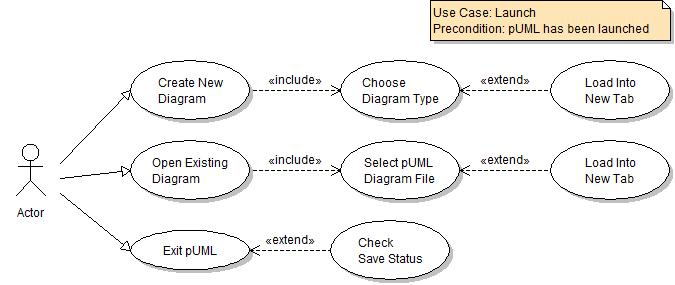
\includegraphics[width=6.0in]{ucaseLaunch.jpg}
\end{figure}



\begin{flushleft}
\tablehead{}
\begin{tabular}{|m{2.0in} m{5.0in}|}
\hline
{\selectlanguage{english}\bfseries\color{black}\emph{Use Case Name}}
&
{\selectlanguage{english}\bfseries\color{black}
Run Program
}
\\\hline
\emph{
Details
}
&
TBD
\\\hline
\end{tabular}
\end{flushleft}

\bigskip

\begin{flushleft}
\tablehead{}
\begin{tabular}{|m{2.0in} m{5.0in}|}
\hline
{\selectlanguage{english}\bfseries\color{black}\emph{Use Case Name}}
&
{\selectlanguage{english}\bfseries\color{black}
Create New Project
}
\\\hline
\emph{
Details
}
&
TBD
\\\hline
\end{tabular}
\end{flushleft}

\bigskip

\begin{flushleft}
\tablehead{}
\begin{tabular}{|m{2.0in} m{5.0in}|}
\hline
{\selectlanguage{english}\bfseries\color{black}\emph{Use Case Name}}
&
{\selectlanguage{english}\bfseries\color{black}
Open Project
}
\\\hline
\emph{
Details
}
&
TBD
\\\hline
\end{tabular}
\end{flushleft}

\bigskip

\begin{flushleft}
\tablehead{}
\begin{tabular}{|m{2.0in} m{5.0in}|}
\hline
{\selectlanguage{english}\bfseries\color{black}\emph{Use Case Name}}
&
{\selectlanguage{english}\bfseries\color{black}
New Diagram
}
\\\hline
\emph{
Participating Actor
}
&
User
\\\hline
\multirow{2}{*}{\emph{
Flow of Events
}}
& 1.  The user selects new file from menu \\
& 2.  Program requests user select a diagram type
(includes ChooseDiagramType use case) \\
& 3.  The program responds by creating a new file with a blank drawing canvas
\\\hline
\emph{
Entry Condition
}
&
User selects New File from commands
\\\hline
\emph{
Exit Condition
}
&
Program successfully opens new file
\\\hline
\emph{
Quality Requirements
}
&
TBD
\\\hline
\end{tabular}
\end{flushleft}

\bigskip

\begin{flushleft}
\tablehead{}
\begin{tabular}{|m{2.0in} m{5.0in}|}
\hline
{\selectlanguage{english}\bfseries\color{black}\emph{Use Case Name}}
&
{\selectlanguage{english}\bfseries\color{black}
Choose Diagram Type}
\\\hline
\emph{
Participating Actor
}
&
User
\\\hline
\multirow{2}{*}{\emph{
Flow of Events
}}
& 1.  User selects a diagram type \\
& 2.  Program loads and displays only objects for the selected diagram type
\\\hline
\emph{
Entry Condition
}
&
Included from New Diagram use case
\\\hline
\emph{
Exit Condition
}
&
Included from New Diagram use case
\\\hline
\emph{
Quality Requirements
}
&
TBD
\\\hline
\end{tabular}
\end{flushleft}

\bigskip


\begin{flushleft}
\tablehead{}
\begin{tabular}{|m{2.0in} m{5.0in}|}
\hline
{\selectlanguage{english}\bfseries\color{black}\emph{Use Case Name}}
&
{\selectlanguage{english}\bfseries\color{black}
Open Diagram}
\\\hline
\emph{
Participating Actor
}
&
User
\\\hline
\multirow{2}{*}{\emph{
Flow of Events
}}
& 1. User selects Open File from menu \\
& 2. Program opens an explorer window \\
& 3. User selects a file \\
& 4. Program loads selected file into program \\\hline
\emph{
Entry Condition
}
&
User selects Open File from menu.
\\\hline
\emph{
Exit Condition
}
&
File is successfully opened.
\\\hline
\emph{
Quality Requirements
}
&
User selected file must be able to be opened in pUML.
\\\hline
\end{tabular}
\end{flushleft}

\bigskip

\begin{flushleft}
\tablehead{}
\begin{tabular}{|m{2.0in} m{5.0in}|}
\hline
{\selectlanguage{english}\bfseries\color{black}\emph{Use Case Name}}
&
{\selectlanguage{english}\bfseries\color{black}
Close Program}
\\\hline
\emph{
Participating Actor
}
&
User
\\\hline
\multirow{2}{*}{\emph{
Flow of Events
}}
& 1. User clicks X \\
& 2. If file is not saved, include Save File As use case \\
& 3. Program Exits \\\hline
\emph{
Entry Condition
}
&
User initiates File menu option Close Program or clicks X in the corner of the window.
\\\hline
\emph{
Exit Condition
}
&
File is successfully saved and the program exits.
\\\hline
\emph{
Quality Requirements
}
&
TBD
\\\hline
\end{tabular}
\end{flushleft}





\bigskip
\bigskip



\paragraph[\ Use Category]
{\ Running} {\selectlanguage{english}\color{black}
These options will be available to the user if a project has been opened.  This case inherits all options from Launch.
}

\bigskip
\bigskip

\begin{figure}[h]
\centering
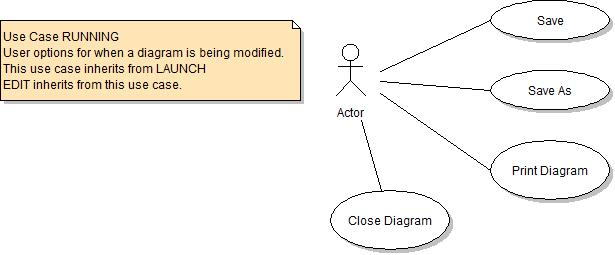
\includegraphics[width=6.0in]{ucaseRunning.jpg}
\end{figure}

\begin{flushleft}
\tablehead{}
\begin{tabular}{|m{2.0in} m{5.0in}|}
\hline
{\selectlanguage{english}\bfseries\color{black}\emph{Use Case Name}}
&
{\selectlanguage{english}\bfseries\color{black}
Save File}
\\\hline
\emph{
Participating Actor
}
&
User
\\\hline
\multirow{2}{*}{\emph{
Flow of Events
}}
& 1. The user selects save file \\
& 2. Program saves file \\
& a. If file has not been previously saved, ask user where to save \\
& b. If file has been previously saved, ask user where to save
\\\hline
\emph{
Entry Condition
}
&
User selects Save File from main menu or clicks save button.
\\\hline
\emph{
Exit Condition
}
&
File is successfully saved
\\\hline
\emph{
Quality Requirements
}
&
TBD
\\\hline
\end{tabular}
\end{flushleft}

\bigskip

\begin{flushleft}
\tablehead{}
\begin{tabular}{|m{2.0in} m{5.0in}|}
\hline
{\selectlanguage{english}\bfseries\color{black}\emph{Use Case Name}}
&
{\selectlanguage{english}\bfseries\color{black}
Save As
}
\\\hline
\emph{
Details
}
&
TBD
\\\hline
\end{tabular}
\end{flushleft}

\bigskip


\begin{flushleft}
\tablehead{}
\begin{tabular}{|m{2.0in} m{5.0in}|}
\hline
{\selectlanguage{english}\bfseries\color{black}\emph{Use Case Name}}
&
{\selectlanguage{english}\bfseries\color{black}
Print Diagram}
\\\hline
\emph{
Participating Actor
}
&
User
\\\hline
\multirow{2}{*}{\emph{
Flow of Events
}}
& 1.  User initiates print. \\
& 2.  Program sends to printer
\\\hline
\emph{
Entry Condition
}
&
User initiates Print
\\\hline
\emph{
Exit Condition
}
&
Diagram successfully sent to printer
\\\hline
\emph{
Quality Requirements
}
&
TBD
\\\hline
\end{tabular}
\end{flushleft}

\bigskip

\begin{flushleft}
\tablehead{}
\begin{tabular}{|m{2.0in} m{5.0in}|}
\hline
{\selectlanguage{english}\bfseries\color{black}\emph{Use Case Name}}
&
{\selectlanguage{english}\bfseries\color{black}
Close Diagram
}
\\\hline
\emph{
Details
}
&
TBD
\\\hline
\end{tabular}
\end{flushleft}

\bigskip
\bigskip

\paragraph[\ Use Category]
{\ Editing} {\selectlanguage{english}\color{black}
These options will be available to the user while ediiting a UML diagram.  This case inherits all use cases from Launch and Running.
}

\bigskip
\bigskip

\begin{figure}[h]
\centering
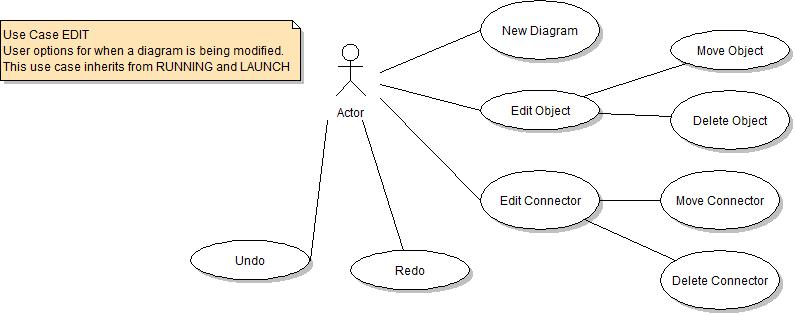
\includegraphics[width=6.0in]{ucaseEdit.jpg}
\end{figure}

\bigskip

\begin{flushleft}
\tablehead{}
\begin{tabular}{|m{2.0in} m{5.0in}|}
\hline
{\selectlanguage{english}\bfseries\color{black}\emph{Use Case Name}}
&
{\selectlanguage{english}\bfseries\color{black}
Create New Object
}
\\\hline
\emph{
Participating Actor
}
&
User
\\\hline
\multirow{2}{*}{\emph{
Flow of Events
}}
& 1.  User selects an object from a valid list of objects \\
& 2.  User places object on canvas.
\\\hline
\emph{
Entry Condition
}
&
Toolbar is loaded with valid objects for diagram type
\\\hline
\emph{
Exit Condition
}
&
Object has been successfully placed on drawing canvas.
\\\hline
\emph{
Quality Requirements
}
&
TBD
\\\hline
\end{tabular}
\end{flushleft}

\bigskip

\begin{flushleft}
\tablehead{}
\begin{tabular}{|m{2.0in} m{5.0in}|}
\hline
{\selectlanguage{english}\bfseries\color{black}\emph{Use Case Name}}
&
{\selectlanguage{english}\bfseries\color{black}
Edit Object
}
\\\hline
\emph{
Details
}
&
TBD
\\\hline
\end{tabular}
\end{flushleft}

\bigskip

\begin{flushleft}
\tablehead{}
\begin{tabular}{|m{2.0in} m{5.0in}|}
\hline
{\selectlanguage{english}\bfseries\color{black}\emph{Use Case Name}}
&
{\selectlanguage{english}\bfseries\color{black}
Edit Connector
}
\\\hline
\emph{
Details
}
&
TBD
\\\hline
\end{tabular}
\end{flushleft}

\bigskip



\begin{flushleft}
\tablehead{}
\begin{tabular}{|m{2.0in} m{5.0in}|}
\hline
{\selectlanguage{english}\bfseries\color{black}\emph{Use Case Name}}
&
{\selectlanguage{english}\bfseries\color{black}
Undo
}
\\\hline
\emph{
Details
}
&
TBD
\\\hline
\end{tabular}
\end{flushleft}

\bigskip


\begin{flushleft}
\tablehead{}
\begin{tabular}{|m{2.0in} m{5.0in}|}
\hline
{\selectlanguage{english}\bfseries\color{black}\emph{Use Case Name}}
&
{\selectlanguage{english}\bfseries\color{black}
Redo
}
\\\hline
\emph{
Details
}
&
TBD
\\\hline
\end{tabular}
\end{flushleft}

\bigskip

\clearpage




\subsubsection[System feature: [Project management tasks suite]{\selectlanguage{english}\rmfamily\bfseries\color{black} System
feature: Project management tasks suite}

\paragraph[\ Introduction/Purpose of this feature]{\foreignlanguage{english}{\ }\foreignlanguage{english}{Introduction/Purpose of this feature}}
{\selectlanguage{english}\color{black}
Several processes are required to manage projects. These include the saving of files, loading projects from files, and deleting projects.}


\paragraph[Input/Output sequence for this feature]{\selectlanguage{english}\rmfamily\bfseries\color{black}
Input/Output sequence for this feature}
{\selectlanguage{english}\color{black}
The user selects the "File" pull down menu at the top left corner of his or her screen. The options currently supported are "New", "Open", "Revert", "Copy As", "Save", "Save As", and "Delete Project". }

\subparagraph{New}
{\selectlanguage{english}\color{black}
This creates a new project space. The user shall be presented with a dialog option to save the previous project. Once completing this dialog, the previous project will be closed and a new project space will be created. }

\subparagraph{Open}
{\selectlanguage{english}\color{black}
This opens a previously saved project. The user shall be presented with a dialog option to save the previous project. Once completing this dialog, the previous project will be closed and the selected project will be opened.}

\subparagraph{Revert}
{\selectlanguage{english}\color{black}
This disregards all unsaved changes made to the project and reverts to the saved version. A confirmation dialog shall be presented to the user before this action is completed.}

\subparagraph{Copy As}
{\selectlanguage{english}\color{black}
This creates a new project space. First, the program will be saved. Then the user shall be presented with a dialog to choose a unique name for the new project space. Once completing this dialog, a copy of the previous project will be cloned into the new project space. The previous project shall be closed and the new project shall be opened.}

\subparagraph{Save}
{\selectlanguage{english}\color{black}
This saves the current state of the project into an XML that can later be used to recreate the project state. If the current project does not have a name, the "Save" option will be an alias for the "Save As" option.}

\subparagraph{Save As}
{\selectlanguage{english}\color{black}
This creates a new project space and then saves the project state into the new project. In contrast with "Copy As", this option does not affect the previous project. }

\subparagraph{Delete Project}
{\selectlanguage{english}\color{black}
This deletes the current project and all files within the project folder. The user shall be presented with a confirmation dialog before this action is completed. Upon completion, a blank and unnamed project will be active in the project window. }









\clearpage\setcounter{page}{1}\pagestyle{Convertvi}
\section[REQUIREMENTS TRACEABILITY]{\selectlanguage{english}\rmfamily\bfseries\color{black}
REQUIREMENTS TRACEABILITY}
{\selectlanguage{english}\itshape\color{black}
This section shall contain traceability information from each system
requirement in this specification to the system (or subsystem, if
applicable) requirements it addresses. \ A tabular form is preferred,
but not mandatory.}


\bigskip

\begin{flushleft}
\tablehead{\hline
\multicolumn{1}{|m{0.9212598in}|}{\centering
\selectlanguage{english}\bfseries\color{black} Feature Name} &
\centering \selectlanguage{english}\bfseries\color{black} Req No. &
\centering \selectlanguage{english}\bfseries\color{black} Requirement
Description &
\centering \selectlanguage{english}\bfseries\color{black} Priority &
\centering \selectlanguage{english}\bfseries\color{black} SDD &
\multicolumn{2}{m{1.2872598in}|}{\centering
\selectlanguage{english}\bfseries\color{black} Alpha Release} &
\multicolumn{2}{m{1.3587599in}|}{\centering
\selectlanguage{english}\bfseries\color{black} Beta Release} &
\multicolumn{2}{m{1.3795599in}|}{\centering
\selectlanguage{english}\bfseries\color{black} Final Test}\\\hline
 &
 &
 &
 &
 &
\centering \selectlanguage{english}\bfseries\color{black} Test Case(s) &
\centering \selectlanguage{english}\bfseries\color{black} Test Res. &
\centering \selectlanguage{english}\bfseries\color{black} Test Case(s) &
\centering \selectlanguage{english}\bfseries\color{black} Test Res. &
\centering \selectlanguage{english}\bfseries\color{black} Test Case(s) &
\selectlanguage{english}\bfseries\color{black} Test
Res.\\\hhline{~~~~~------}}
\begin{supertabular}{m{0.9212598in}|m{0.42125985in}|m{1.9212599in}|m{0.39275986in}|m{0.7587598in}|m{0.6622598in}|m{0.5462598in}|m{0.6712598in}|m{0.6087598in}|m{0.6712598in}|m{0.6295598in}|}
\multicolumn{1}{|m{0.9212598in}|}{~Select Diagram Type
} &
\centering \selectlanguage{english}\color{black} 1.1 &
~Selects the appropriate diagram type
 &
~M
 &
~N/A
 &
~N/A
 &
~N/A
 &
~N/A
 &
~N/A
 &
~N/A
 &

~N/A
\\\hline
\multicolumn{1}{|m{0.9212598in}|}{~Save function
} &
\centering \selectlanguage{english}\color{black} 2.1 &
~Saves the Diagram to file
 &
~M
 &
~N/A
 &
~N/A
 &
~N/A
 &
~N/A
 &
~N/A
 &
~N/A
 &
~N/A
 
\\\hline
\multicolumn{1}{|m{0.9212598in}|}{~Draw function
} &
\centering \selectlanguage{english}\color{black} 2.1 &
~Draws current objects
 &
~M
 &
~N/A
 &
~N/A
 &
~N/A
 &
~N/A
 &
~N/A
 &
~N/A
 &
~N/A

\\\hline
\multicolumn{1}{|m{0.9212598in}|}{~Open File
} &
\centering \selectlanguage{english}\color{black} 2.1 &
~Opens previously saved file
 &
~M
 &
~N/A
 &
~N/A
 &
~N/A
 &
~N/A
 &
~N/A
 &
~N/A
 &
~N/A

\\\hline
\multicolumn{1}{|m{0.9212598in}|}{~New File
} &
\centering \selectlanguage{english}\color{black} 2.1 &
~Creates New File
 &
~M
 &
~N/A
 &
~N/A
 &
~N/A
 &
~N/A
 &
~N/A
 &
~N/A
 &
~N/A

\\\hline

\multicolumn{1}{|m{0.9212598in}|}{~SSRS and SSDD
} &
\centering \selectlanguage{english}\color{black} 2.1 &
~Too much work.
 &
~M
 &
~N/A
 &
~N/A
 &
~N/A
 &
~N/A
 &
~N/A
 &
~N/A
\\\hline

\end{supertabular}
\end{flushleft}
{\selectlanguage{english}\color{black}
Priorities are: \textbf{M}andatory, \textbf{L}ow, \textbf{H}igh}

{\selectlanguage{english}\color{black}
SDD link is version and page number or function name.}

{\selectlanguage{english}\color{black}
Test cases and results are file names and \textbf{P}ass/\textbf{F}ail or
\% passing.}


\end{document}